% This is "sig-alternate.tex" V2.1 April 2013
% This file should be compiled with V2.5 of "sig-alternate.cls" May 2012
%
% This example file demonstrates the use of the 'sig-alternate.cls'
% V2.5 LaTeX2e document class file. It is for those submitting
% articles to ACM Conference Proceedings WHO DO NOT WISH TO
% STRICTLY ADHERE TO THE SIGS (PUBS-BOARD-ENDORSED) STYLE.
% The 'sig-alternate.cls' file will produce a similar-looking,
% albeit, 'tighter' paper resulting in, invariably, fewer pages.
%
% ----------------------------------------------------------------------------------------------------------------
% This .tex file (and associated .cls V2.5) produces:
%       1) The Permission Statement
%       2) The Conference (location) Info information
%       3) The Copyright Line with ACM data
%       4) NO page numbers
%
% as against the acm_proc_article-sp.cls file which
% DOES NOT produce 1) thru' 3) above.
%
% Using 'sig-alternate.cls' you have control, however, from within
% the source .tex file, over both the CopyrightYear
% (defaulted to 200X) and the ACM Copyright Data
% (defaulted to X-XXXXX-XX-X/XX/XX).
% e.g.
% \CopyrightYear{2007} will cause 2007 to appear in the copyright line.
% \crdata{0-12345-67-8/90/12} will cause 0-12345-67-8/90/12 to appear in the copyright line.
%
% ---------------------------------------------------------------------------------------------------------------
% This .tex source is an example which *does* use
% the .bib file (from which the .bbl file % is produced).
% REMEMBER HOWEVER: After having produced the .bbl file,
% and prior to final submission, you *NEED* to 'insert'
% your .bbl file into your source .tex file so as to provide
% ONE 'self-contained' source file.
%
% ================= IF YOU HAVE QUESTIONS =======================
% Questions regarding the SIGS styles, SIGS policies and
% procedures, Conferences etc. should be sent to
% Adrienne Griscti (griscti@acm.org)
%
% Technical questions _only_ to
% Gerald Murray (murray@hq.acm.org)
% ===============================================================
%
% For tracking purposes - this is V2.0 - May 2012

\documentclass{sig-alternate-05-2015}

% Redefines \@ptsize to make setspace happy
\makeatletter
\renewcommand{\@ptsize}{0}
\makeatother

\usepackage{ig}
\usepackage{setspace}
\doublespacing

\begin{document}

% Copyright
\setcopyright{acmcopyright}
%\setcopyright{acmlicensed}
%\setcopyright{rightsretained}
%\setcopyright{usgov}
%\setcopyright{usgovmixed}
%\setcopyright{cagov}
%\setcopyright{cagovmixed}


% DOI
\doi{10.475/123_4}

% ISBN
\isbn{123-4567-24-567/08/06}

%Conference
\conferenceinfo{PLDI '13}{June 16--19, 2013, Seattle, WA, USA}

\acmPrice{\$15.00}

%
% --- Author Metadata here ---
\conferenceinfo{WOODSTOCK}{'97 El Paso, Texas USA}
%\CopyrightYear{2007} % Allows default copyright year (20XX) to be over-ridden - IF NEED BE.
%\crdata{0-12345-67-8/90/01}  % Allows default copyright data (0-89791-88-6/97/05) to be over-ridden - IF NEED BE.
% --- End of Author Metadata ---

\title{A Domain-Specific Programming Language for Robots based on Instruction
  Graphs
}

%
% You need the command \numberofauthors to handle the 'placement
% and alignment' of the authors beneath the title.
%
% For aesthetic reasons, we recommend 'three authors at a time'
% i.e. three 'name/affiliation blocks' be placed beneath the title.
%
% NOTE: You are NOT restricted in how many 'rows' of
% "name/affiliations" may appear. We just ask that you restrict
% the number of 'columns' to three.
%
% Because of the available 'opening page real-estate'
% we ask you to refrain from putting more than six authors
% (two rows with three columns) beneath the article title.
% More than six makes the first-page appear very cluttered indeed.
%
% Use the \alignauthor commands to handle the names
% and affiliations for an 'aesthetic maximum' of six authors.
% Add names, affiliations, addresses for
% the seventh etc. author(s) as the argument for the
% \additionalauthors command.
% These 'additional authors' will be output/set for you
% without further effort on your part as the last section in
% the body of your article BEFORE References or any Appendices.

\numberofauthors{1} %  in this sample file, there are a *total*
% of EIGHT authors. SIX appear on the 'first-page' (for formatting
% reasons) and the remaining two appear in the \additionalauthors section.
%
\author{
% You can go ahead and credit any number of authors here,
% e.g. one 'row of three' or two rows (consisting of one row of three
% and a second row of one, two or three).
%
% The command \alignauthor (no curly braces needed) should
% precede each author name, affiliation/snail-mail address and
% e-mail address. Additionally, tag each line of
% affiliation/address with \affaddr, and tag the
% e-mail address with \email.
%
% 1st. author
\alignauthor
Andrew Benson\titlenote{Only the student author is listed here for this written
  report. The author also wishes to credit Jonathan Aldrich, Joshua Sunshine,
  and Cyrus Omar for their contributions.}\\
       \affaddr{Computer Science Department}\\
       \affaddr{Carnegie Mellon University}\\
       \affaddr{Pittsburgh, USA}\\
       \email{adbenson@andrew.cmu.edu}
}

% There's nothing stopping you putting the seventh, eighth, etc.
% author on the opening page (as the 'third row') but we ask,
% for aesthetic reasons that you place these 'additional authors'
% in the \additional authors block, viz.
% Just remember to make sure that the TOTAL number of authors
% is the number that will appear on the first page PLUS the
% number that will appear in the \additionalauthors section.

\maketitle
\begin{abstract}
Instruction graphs are a recently proposed data structure that encodes a
sequence of actions for a robot to perform \cite{veloso:instructiongraphs}. For
example, in order for a robot to purchase coffee, a robot might move forward,
looking for a barista every 5 meters, then ask for a coffee once a barista is
found. An instruction graph is an explicit representation of these actions,
where each action is a vertex and edges are the transitions between them. We
contribute a formalization of instruction graphs as a domain-specific
programming language, prove type safety for the language, and provide an
interpreter.
\end{abstract}

%
% The code below should be generated by the tool at
% http://dl.acm.org/ccs.cfm
% Please copy and paste the code instead of the example below. 
%
 \begin{CCSXML}
<ccs2012>
<concept>
<concept_id>10010520.10010553.10010554.10010556</concept_id>
<concept_desc>Computer systems organization~Robotic control</concept_desc>
<concept_significance>300</concept_significance>
</concept>
<concept>
<concept_id>10011007.10011006.10011050.10011017</concept_id>
<concept_desc>Software and its engineering~Domain specific languages</concept_desc>
<concept_significance>300</concept_significance>
</concept>
</ccs2012>
\end{CCSXML}

\ccsdesc[300]{Computer systems organization~Robotic control}
\ccsdesc[300]{Software and its engineering~Domain specific languages}

%
% End generated code
%

%
%  Use this command to print the description
%
\printccsdesc

% We no longer use \terms command
%\terms{Theory}

\keywords{Instruction Graphs; Robotic Domain Specific Languages}

\section{Instruction Graphs}
Being able to follow sequences of actions is a very important function of a
robot. Many tasks that a robot is programmed to do are already in the form of
a sequence of actions. For example, there is a very natural sequence of actions
a robot might do in order to navigate a maze - turn left, move forward five
meters, turn right, etc. Some tasks may also involve conditional actions, so
that the robot may branch in its execution of actions dependent on some
environmental condition. For example, instead of traveling a predetermined five
meters forward, a robot might move forward until it senses a wall a meter away.
We are interested in this set of tasks that can be expressed as a composition of
primitive robotic actions.

Instruction graphs are a recently proposed data structure by which such tasks
can be encoded and expressed \cite{veloso:instructiongraphs}. Informally, an
instruction graph consists of vertices, which can be thought of as actions a
robot might do like ``move forward five meters'' or conditions a robot may check
like ``is there a wall one meter away'', and edges, which connect the actions in
a sequence or in a branching pattern (in the case of a conditional vertex).
Instruction graphs distinguish four classes of vertices: \textbf{Do} vertices,
which represent a single action executed once; \textbf{DoUntil} vertices,
which represent an action executed until a condition is met;
\textbf{Conditional} vertices, which represent a condition to be checked to
determine which vertex to proceed to; and \textbf{GoTo} vertices, which
merely represent an advancement to another vertex and are usually used only to
implement loops.

Instruction graphs have already been detailed and used in other research. In
\cite{veloso:instructiongraphs}, instruction graphs are generated by a robot
by parsing natural language whenever a user verbally specifies a task to the
robot. However, most of the attention was focused on the spoken interaction
between the human and robot and how the instruction graph is generated.
Instruction graphs were an internal detail of the robot and could not be created
unless generated via spoken interaction with the robot.

\section{Approach}

Our goal in this research is to explore the capabilities of instruction graphs
and to formalize their creation and execution. We have three main contributions
to make in this direction:

\begin{itemize}
  \item Formalization of instruction graphs as a domain-specific programming
    language - the instruction graph language
  \item Proof of type safety for this language
  \item Interpreter for the instruction graph language on the Turtlebot
    simulator
\end{itemize}

For the first point, we formalize instruction graphs into a programming language
by giving a grammar, specifying what it means to be well-formed by detailing
statics, and specifying its execution through a description of its dynamics.

For the second point, we first define theorems of progress and preservation for
the language, then prove them to ensure that the language is safe.

For the third point, we write a lexer and parser to read concrete programs of
the language, check statics on the program, and interpret the program as
specified by the dynamics. We demonstrate the feasibility of the language by
simulating the execution of the program in the Turtlebot simulator.

\section{Instruction Graph Language}

Before formally specifying the language via its grammar, statics, and dynamics,
it is helpful to see an example of an instruction graph and its corresponding
program in the instruction graph language.

\subsection{The ``Get Coffee'' Program}

\begin{figure}
\centering
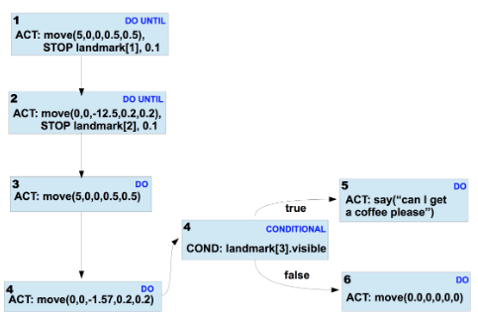
\includegraphics[height=2.233in, width=3.346in]{images/getcoffee-ig.png}
\caption{The instruction graph for the ``get coffee'' program.}
\end{figure}

In Figure 1 we see the instruction graph representing a robot's task to get
coffee. Admittedly, the task itself is a bit contrived. The robot begins by
moving with parameters (5, 0, 0, 0.5, 0.5) (the meaning of the parameters is
unknown without knowing more about the robot, but one could guess that it
specifies at least speed, distance, and rotation) until it is within 0.1 meters
of landmark[1], then changes direction and moves with parameters (0, 0, -12.5,
0.2, 0.2) until it is within 0.1 meters of landmark[2]. Then it moves with
parameters (5, 0, 0, 0.5, 0.5) and then with parameters (0, 0, -1.57, 0.2, 0.2).
Following that, it checks whether landmark[3] is visible, and if so, it says
``can I get a coffee please'', otherwise moves with parameters (0, 0, 0, 0, 0).

With this instruction graph we can see most of the features present in
instruction graphs - \textbf{Do} vertices, \textbf{DoUntil} vertices,
\textbf{Conditional} vertices, move actions, condition checking, etc. We miss
seeing \textbf{GoTo} vertices, but those are very straightforward - the robot
simply moves to the next vertex.

\begin{figure}
\centering
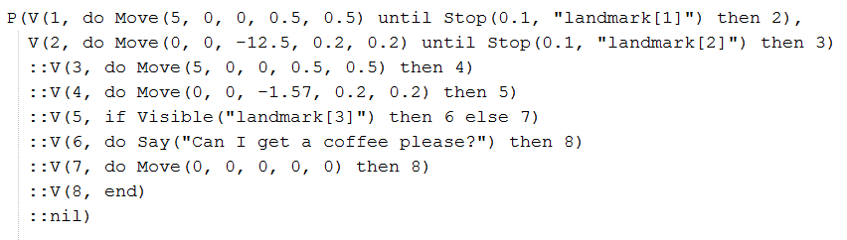
\includegraphics[height=1.2in, width=3.8115in]{images/getcoffee-igprog.png}
\caption{The corresponding instruction graph program for the ``get coffee''
  program.}
\end{figure}

In Figure 2 we see the corresponding instruction graph program for getting
coffee. The similarity between the instruction graph and the instruction graph
program should be quite clear.

\subsection{Discussion of Grammar}

\begin{figure*}
\centering
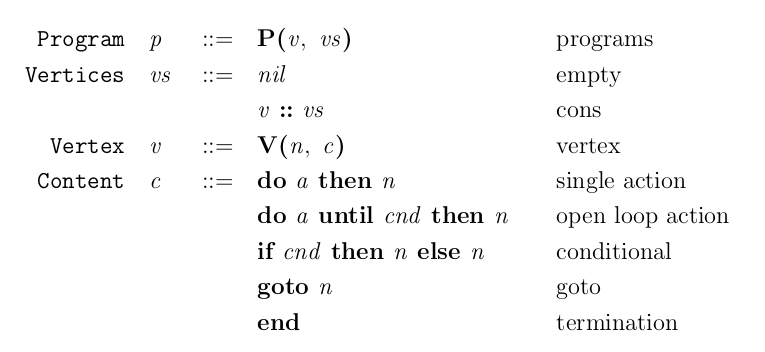
\includegraphics[height=2.35in, width=5.1in]{images/grammar.png}
\caption{Grammar for the instruction graph language.}
\end{figure*}

As can be seen from inspecting the structure of the example program above,
programs written in the instruction graph language are quite simple and closely
follow the layout of an instruction graph. Informally, programs consist of a
start vertex and a list of all other vertices in the program, all of which are
given an index to identify them. Each vertex is one of the classes discussed
earlier - \textbf{Do}, \textbf{DoUntil}, \textbf{Conditional}, or \textbf{GoTo}
- and contains the appropriate content (action or condition or neither) for its
class. The exception is \textbf{End}, which signals that this vertex is the last
vertex to be executed in the program. Each vertex also lists the possible
vertices that could follow it during execution.

Figure 3 shows the grammar for the instruction graph language. Note that a few
parts of the language have been omitted from this grammar. Firstly, note that
$n \in \mathbb{Z}$, the integers. Secondly, since the actions and conditions
that a particular robot could respectively do or check varies by the robot, a
grammar for them has been omitted. The actions $a$ and conditions $c$ still
need to be well-specified by the implementor, though. For instance, for the
particular robot the ``get coffee'' program above was written for, actions $a$
can be either Move, which takes in five floats as arguments, or Say, which takes
a string as an argument.

It is worth noting that the instruction graph language is unlike most
programming languages. Programs in this language are not traditional expressions
that can be evaluated to model a mathematical function, as in most languages,
but are descriptions of graphs. This language also has no types or values, at
least in the traditional sense, but has many side-effects, which is opposite
most programming languages. It is worth emphasizing that the instruction graph
language is a \textit{domain specific language} for specifying tasks to robots,
not a general purpose programming language, so the language should be expected
to look and behave differently from conventional programming languages.

\section{Statics}

\begin{figure*}
\centering
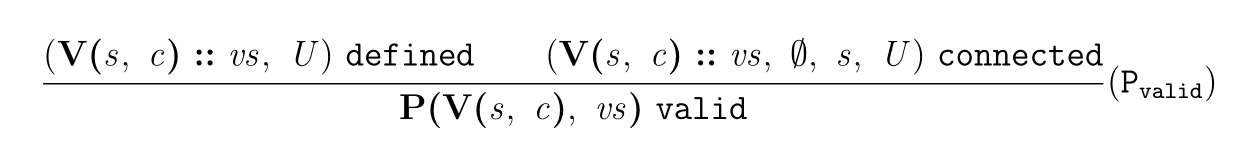
\includegraphics[height=0.75in, width=6in]{images/valid.png}
\caption{Statics: valid judgment.}
\end{figure*}

\begin{figure*}
\centering
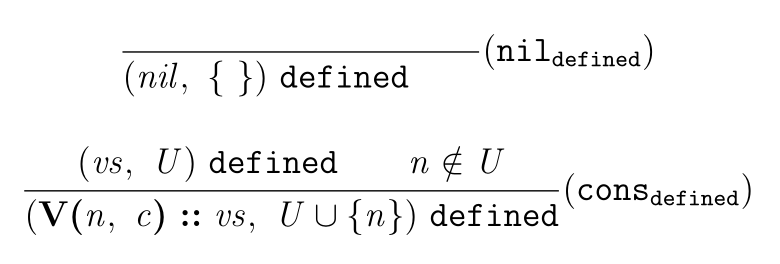
\includegraphics[height=1.3in, width=4in]{images/defined.png}
\caption{Statics: defined judgment.}
\end{figure*}

\begin{figure*}
\centering
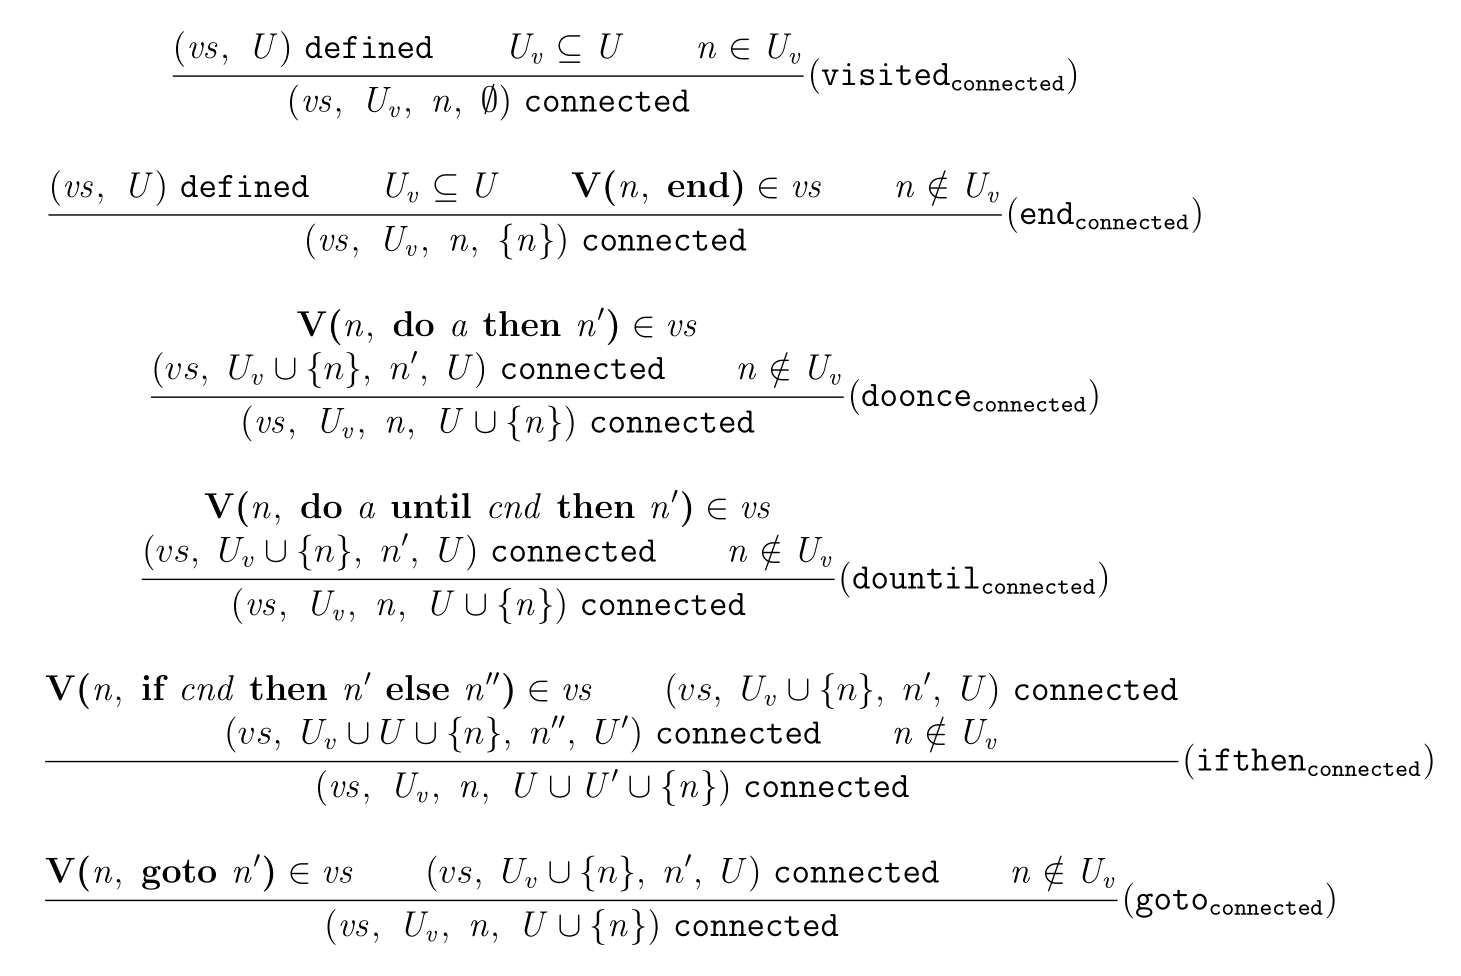
\includegraphics[height=4.5in, width=7in]{images/connected.png}
\caption{Statics: connected judgment.}
\end{figure*}

Most programming languages define statics by giving rules for when expressions
in the language are well-typed. Since the instruction graph language has no
types, the statics are a bit trickier. Fundamentally, though, statics defined
what it means for a program in the language to be well-formed. Thus we can list
several desirable characteristics for programs of this language:

\begin{itemize}
  \item No two vertices should have the same index.
  \item Every vertex that follows another vertex should be defined.
  \item There should exist a path from the start vertex to every defined vertex.
\end{itemize}

Since programs can be thought of as descriptions of graphs, these
characteristics make intuitive sense when considering them as so. The first item
thus states that no vertex is defined twice. The second says that every edge
should connect to a defined vertex. The third expresses the idea that the
instruction graph that the program represents should be a connected graph.

When all of these conditions are met, we consider the program to be a valid one.
We formally judge a program to be valid using the judgment shown in Figure 4. In
other words, a program is valid when it defines a set of vertex indices $U$, and
the start vertex is connected to exactly the vertices in $U$.

Of course, we must define what it means to be defined and connected as well.
Those are formally shown in Figures 5 and 6.

Informally, a program defines a set $U$ of vertex indices if its list of
vertices only defines each vertex once and each vertex index in the list appears
in U and vice versa.

The connected judgment is more tricky. The idea is to do a BFS search from the
start vertex outward, keeping track of which vertices have been visited, and
discovering which vertices are connected that haven't been visited.

The appendix reproduces the statics and explains them in more detail as well.

\section{Dynamics}

\begin{figure*}
\centering

\includegraphics[height=0.35in, width=4in]{images/configuration.png}
\caption{Dynamics: configuration definition.}
\end{figure*}

\begin{figure*}
\centering
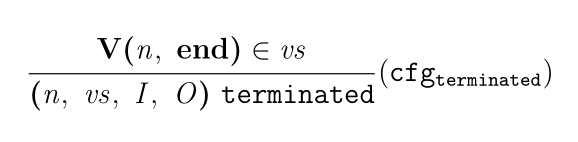
\includegraphics[height=0.8in, width=3in]{images/terminated.png}
\caption{Dynamics: terminated judgment.}
\end{figure*}

\begin{figure*}
\centering
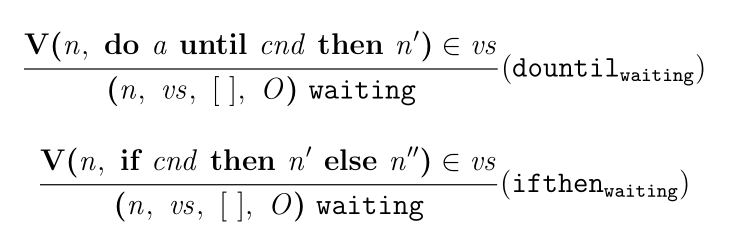
\includegraphics[height=1.4in, width=4in]{images/waiting.png}
\caption{Dynamics: waiting judgment.}
\end{figure*}

\begin{figure*}
\centering
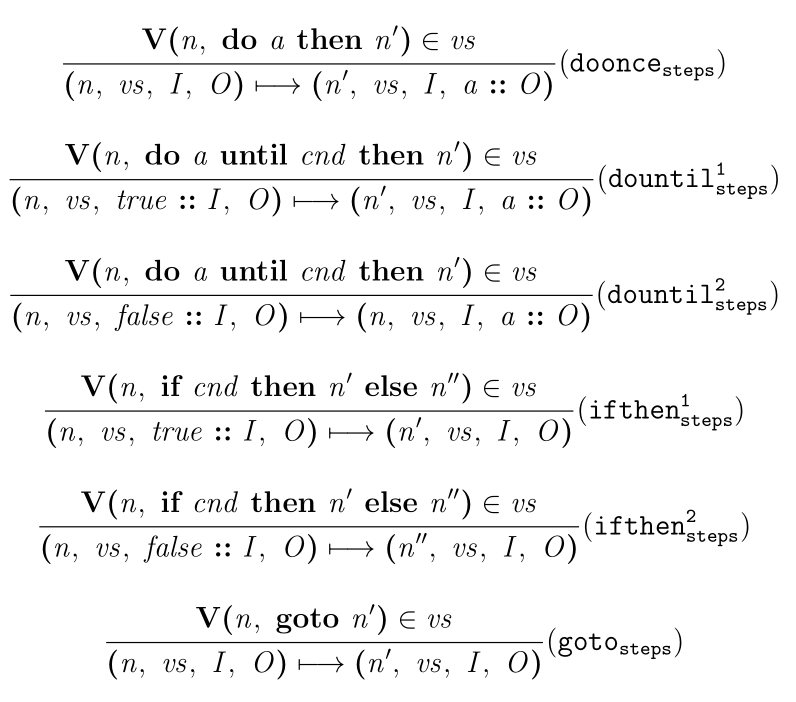
\includegraphics[height=3.5in, width=4in]{images/steps.png}
\caption{Dynamics: steps judgment.}
\end{figure*}

To write dynamics for the instruction graph language we need a machine model for
how programs in the language are evaluated and executed. Intuitively, this is
clear - begin at the vertex representing the start vertex, execute its action,
and continue as directed until we hit \textbf{End}. But to be precise and
rigorous, we have to also keep track of both the inputs to the program i.e.
whether the conditions the robot checks are true and the outputs of the program
i.e. the actions executed.

To that end we define a \textit{configuration} which is a 4-tuple that describes
the state of a program midway through execution. It consists of the index $n$ of
the current vertex being considered, the list $vs$ of all vertices in the
program, the list $I$ of inputs to the program, and the list $O$ of outputs of
the program.

A configuration is defined formally in Figure 7.

\clearpage

Ideally, whenever an instruction graph program is executing, one of two things
is true: either the program has ended i.e. $n$ points to a vertex that has
\textbf{End} as its content, or the program can continue executing i.e. there's
a new configuration that the program can proceed to. However, there is actually
a third possibility. Since the input to the program was specified as a list, the
formal execution of a program could accidentally ``run out of inputs'' if the
list of inputs is empty. In practice, this should never happen unless the robot
is malfunctioning, as there is no reason why the robot cannot check a condition
to receive input. Because we are forced to deal with this possibility in our
model, we call this state ``waiting'' because it is as if the robot is waiting
for input from its sensors.

We describe a configuration where the program has ended ``terminated'', and we
say that when a program can continue to execute that its configuration
``steps''.

These three judgments are defined precisely in Figures 8-10. They aren't
particularly tricky, but more details on the dynamics are available in the
appendix.

\section{Safety}

In order to be convinced of a language's correctness it is useful to complete a
proof of type safety. Type safety usually deals with progress, which states that
an expression in a language is either a final value or can continue to step,
and preservation, which states that as a well-typed expression steps, it remains
well-typed. Since the ideas of an expression and well-typedness do not apply to
the instruction graph language, proving type safety for the instruction graph
language is not straightforward.

To do so, we must state a variant of progress and preservation that is more
applicable to the ideas of the instruction graph language.

First, though, we should define what a valid configuration is. This is formally
defined in Figure 11. Informally, a valid configuration is one where the
vertices describe a valid program, and the current vertex is one that exists in
the program.

\begin{figure}
\centering
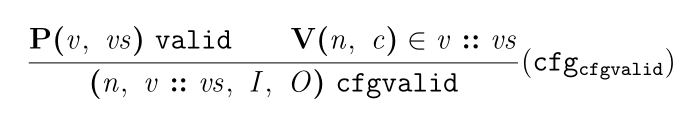
\includegraphics[height=0.65in, width=3.5in]{images/cfgvalid.png}
\caption{Safety: cfgvalid judgment.}
\end{figure}

\newtheorem{theorem}{Safety}
\begin{theorem}
Progress.\\
If $\cfgvalid{\nterm{cfg}}$, then either
\begin{enumerate}
  \item $\terminated{\nterm{cfg}}$
  \item $\waiting{\nterm{cfg}}$
  \item $\exists\ \nterm{cfg'}\ \texttt{s.t.} \steps{\nterm{cfg}}{\nterm{cfg'}}$
\end{enumerate}
\end{theorem}

\begin{theorem}
Preservation.\\
If $\cfgvalid{\nterm{cfg}}$ and $\steps{\nterm{cfg}}{\nterm{cfg'}}$ then
$\cfgvalid{\nterm{cfg'}}$.
\end{theorem}

The formulation of progress comes naturally from the discussion of the dynamics.
A program midway in execution either needs to keep going, be finished, or
perhaps be ``waiting'' due to missing input.

Preservation is quite natural too. If a configuration is valid, stepping it
should neither make the program no longer valid nor step to a vertex that is not
part of the program.

Proving progress and preservation for most languages is long and strenuous. As
such, the proof is omitted here, but the appendix contains the full entirety of
the proof. Instead, we may discuss a basic proof sketch.

The proof for progress is actually not too bad. Given that a configuration is
cfgvalid, the vertex corresponding to $n$ must be part of the program. Next,
case on the structure on this vertex i.e. what its content is, and whether I is
empty or not. As it turns out, every combination of content and whether I is
empty or not directly corresponds to a dynamics rule, so the configuration is
definitely terminated, waiting, or steps to another configuration.

The proof for preservation is more nontrivial. The proof relies on five separate
lemmas, each of which are proved separately. The basic idea is to first
establish that $n$ is connected to some nonempty set of vertices, and from that
show that $n'$ (the vertex $n$ necessarily connects to) is also connected to
some possibly empty set of vertices, which implies that there is a vertex with
that index and thus the configuration is still cfgvalid after stepping. As
usual, the appendix has a more detailed proof of progress and preservation.

\section{Interpreter}

Finally, in order to show that the instruction graph language can work in
practice, we wrote an interpreter that executes instruction graph programs. The
interpreter comprises a lexer and parser, as defined by the grammar, a statics
checker as defined by the statics, and an interpreter that uses the dynamics to
execute the program. In order to simulate the effects of the actions a robot
would make as the program executes, the interpreter hooks into the Turtlebot
simulator, an open source robotics platform running on ROS. The code for the
interpreter, as well as a video demo, can be found at https://github.com/anbenson/instructiongraphs.

\section{Discussion}

\subsection{Surprises}

It is interesting to note how easily a data structure like a graph can be molded
into the confines of a programming language. Although the grammar of the
language is unlike most others, the formulation and implementation of the
statics are almost exactly the same as a breadth-first traversal of the graph to
determine connectiveness. There is a surprising relationship between inference
rules governing invariants and algorithms that take advantage of invariants.

\subsection{Conclusions}

We have proposed a formalization of the instruction graph data structure as a
domain specific programming language, the \textit{instruction graph language}.
Following that, we have proven theorems of type safety for the language. One
consequence of the fact that the instruction graph language is safe is that
because the instruction graph data structure, as evaluated internally by robots
in \cite{veloso:instructiongraphs}, and the instruction graph language are
equivalent, as they both express the same thing, we can extend the theorems of
type safety to the instruction graph data structure. This means that the
instruction graph data structure is safe - execution of it will not get
``stuck'' or transition into an invalid state not predicted by the statics.

We have also created an interpreter to show feasibility of the instruction graph
language.

\subsection{Future Work}

While instruction graphs are expressive enough to describe many robotic tasks,
they are not a particularly pleasant one. There is definitely room for
improvement - for example, the instruction graph language lacks any means of
abstraction. In other words, there is no way to reuse ``subgraphs'' of the
instruction graph in other parts of the instruction graph without copying over
the entire subgraph. Fortunately, further work in instruction graphs should be
made easier by a formalization of instruction graphs, and perhaps by a concrete
interpreter to execute them.

\section{Acknowledgments}
The author would like to thank his advisor, Jonathan Aldrich, for all the advice
and help given throughout this semester-long project. The author would also like
to thank Joshua Sunshine and Cyrus Omar, who also contributed useful feedback
and guidance about this project.

%
% The following two commands are all you need in the
% initial runs of your .tex file to
% produce the bibliography for the citations in your paper.
\bibliographystyle{abbrv}
\bibliography{sigproc}  % sigproc.bib is the name of the Bibliography in this case
% You must have a proper ".bib" file
%  and remember to run:
% latex bibtex latex latex
% to resolve all references
%
% ACM needs 'a single self-contained file'!
%
\end{document}
